\documentclass[11pt]{article}

\usepackage[margin=1in]{geometry}
\usepackage[utf8]{inputenc}
\usepackage[T1]{fontenc}
\usepackage[colorlinks=true,linkcolor=blue!60!black,citecolor=blue!60!black,urlcolor=blue!60!black]{hyperref}
\usepackage{url}
\usepackage{booktabs}
\usepackage{amsfonts}
\usepackage{amsmath}
\usepackage{amssymb}
\usepackage{nicefrac}
\usepackage{microtype}
\usepackage{graphicx}
\usepackage{xcolor}
\usepackage{natbib}
\usepackage{caption}
\usepackage{subcaption}
\emergencystretch=2em

\graphicspath{{figs/}}

\newcommand{\TODO}[1]{\textcolor{red}{\textbf{[TODO: #1]}}}
\newcommand{\FVE}{\mathrm{FVE}}
\newcommand{\ns}{\text{ns}}

\title{What Does Adding a KL Term to a Top-K Sparse Autoencoder\\
Actually Do? A Controlled Decomposition Across Three\\
Selection Mechanisms}

\author{Zach \\ \texttt{zachsvm@gmail.com}}
\date{}

\begin{document}
\maketitle

\begin{abstract}
Variational sparse autoencoders (vSAEs) replace a deterministic Top-K code with
a sampled Gaussian posterior in the hope that the resulting stochasticity
organises features into a better dictionary. We decompose this idea into three
independently testable claims and test each with a pre-registered permutation
battery (5$\sigma$ per comparison, 13 seeds/arm) plus three targeted
dose-response sweeps. \textbf{First}, at the fixed unit variance every public
implementation trains with, the KL term is algebraically an $L_2$ penalty and
no sample is ever drawn; comparing a released vSAE implementation against a
plain Top-K-with-$L_2$-penalty baseline shows a large apparent gap ($d\approx
16$ on reconstruction, $d\approx 13$ on feature liveness), but the gap
decomposes \emph{completely} into five optimiser- and initialisation-side
implementation details --- none of which appears in either the vSAE or the
original Top-K paper's equations --- and vanishes once all five are matched
(all metrics null at the power where every earlier generation of the
comparison was significant at $5\sigma$). \textbf{Second}, once sampling is
switched on, damage is real and large, but it is not a size-of-noise effect on
representation quality: a six-point, 13-seed-per-point dose-response sweep over
the initial noise scale shows reconstruction quality tracking Top-K
\emph{selection instability} almost exactly (Pearson $r=+0.9993$) across a
$12\times$ range of noise. The same near-perfect coupling holds for BatchTopK's
globally-shared selection budget ($r=+0.9979$), ruling out per-token
selection as the cause. It does \emph{not} hold cleanly for JumpReLU's
soft, gradient-learned threshold: an apparently similar naive coupling
($r=+0.9334$) is confounded by an $8\times$ swing in achieved sparsity that
the two hard-$k$ mechanisms cannot exhibit by construction, and controlling
for it weakens the coupling to $r=+0.6297$ ($n=4$), confirmed not to be a
small-sample artifact by doubling the grid density in the confound-controlled
region ($r=+0.5026$, $n=8$). The general lesson is
sharper than ``noise hurts'': the reparameterisation trick is specifically
incompatible with \emph{hard, discrete} selection, and the failure mode of a
\emph{soft} selection mechanism under the same noise is a different one ---
sparsity collapse, not selection churn. \textbf{Third}, every one of the
implementation details in the first claim, run individually as a factor, moves
metrics by $d\approx 5$--$19$ at $5\sigma$ --- the same order of magnitude as,
or larger than, published architectural claims in this literature, none of
them stated in any equation, and a design-level survey of ten SAE-methods
papers (every one cited in our own related work) finds \emph{ten of ten}
report a single training seed per configuration for their headline
results --- a design that cannot express statistical significance for an
architecture-level claim at any effect size. We close with a case study (SAEBench's SCR and
TPP metrics scored against the same two checkpoints, the same dataset, the
same masking grid) where two standard downstream metrics disagree in
direction on whether the vSAE's apparent advantage survives a dictionary-size
control, and report five controls run against that disagreement without
resolving it --- offered as a demonstration of the general problem, not a
verdict on either metric.
\end{abstract}

\section{Introduction}
\label{sec:intro}

Sparse autoencoders (SAEs) decompose language-model activations into an
overcomplete, sparsely-active dictionary of
features~\citep{sharkey2022taking,cunningham2023sparse,bricken2023monosemanticity},
motivated by the observation that individual neurons represent multiple
unrelated concepts in
superposition~\citep{elhage2022superposition}. A natural extension, tried by
several groups independently, is to make the code probabilistic: replace a
point estimate with a variational posterior, as in the variational autoencoder
(VAE)~\citep{kingma2013autoencoding}, and hope that the resulting sampling
noise disperses features that would otherwise collapse onto one another. The
intuition is appealing, cheap to implement --- add a variance head, sample,
add a KL term --- and, as far as we can tell from the released code of every
public vSAE implementation we examined, has never been checked against the
one question that determines whether it can work at all: \emph{does the
sampling noise interact with the discrete Top-K selection step in a way that
could plausibly help, or does it only interact with it in a way that hurts?}

This paper answers that question, and two adjacent ones, with a controlled
experimental decomposition rather than a single end-to-end comparison. We ran
a pre-registered confirmatory battery (13 seeds per arm, permutation tests
with an explicit $p$-value floor reported alongside every result, following
the design discipline of
\citealp{gao2024scalingevaluatingsparseautoencoders}'s own recommendation that
SAE comparisons report seed variance) on a public vSAE
implementation~\citep{marks2024dictionary_learning} against three questions:

\begin{enumerate}
\item \textbf{At the fixed variance every implementation actually trains
  with, is the vSAE distinguishable from a plain Top-K SAE with an $L_2$
  penalty on its activations?} (\S\ref{sec:e1}) They are algebraically
  identical objectives; the empirical question is whether two independent
  implementations of that objective land in the same place after training.
\item \textbf{Once sampling is switched back on, what specifically does the
  noise damage, and does the answer depend on how the sparsity mechanism
  selects features?} (\S\ref{sec:mechanism}) We separate ``does noise hurt''
  (yes, substantially) from ``what is the noise actually doing'' (perturbing
  which features Top-K selects, not degrading the features themselves), and
  test whether that mechanism is specific to per-token Top-K, generalises to
  a mechanism with a globally shared selection budget (BatchTopK), or
  generalises further to a mechanism with no hard cardinality constraint at
  all (JumpReLU).
\item \textbf{Are the effect sizes typically reported for variational SAEs
  distinguishable from the effect sizes of unreported implementation
  choices?} (\S\ref{sec:variance}) We take the five implementation details
  that turned out to matter in question 1 and report their individual effect
  sizes as a lower bound on how large an unremarked implementation choice can
  be in this literature.
\end{enumerate}

\S\ref{sec:e4} then works through a fourth, harder question that does not
resolve as cleanly: whether two standard SAEBench interpretability
metrics~\citep{karvonen2025saebenchcomprehensivebenchmarksparse} --- spurious
correlation removal (SCR) and targeted probe perturbation (TPP) --- agree on
whether a vSAE's apparent advantage over its Top-K baseline survives a
dictionary-size control. They do not, on the same two checkpoints, the same
dataset, the same masking grid, scored the same day. We report five
diagnostics run against that disagreement --- none of which resolves it ---
because the disagreement itself, and our inability to explain it away, is a
useful data point about what these metrics measure, independent of the
vSAE question this paper is otherwise about.

\paragraph{Why a decomposition rather than a benchmark table.} A single
end-to-end comparison between a published vSAE and a published Top-K SAE
answers ``which number is bigger,'' which is not the question anyone actually
wants answered. It cannot distinguish an effect of the KL term from an effect
of five unrelated implementation choices that happen to differ between the two
codebases, and it cannot distinguish ``sampling hurts because of some property
of stochastic latents in general'' from ``sampling hurts because it was tested
against one particular hard-selection mechanism.'' Every claim in this paper
is instead the output of holding everything else fixed and varying one thing:
an implementation detail (\S\ref{sec:e1}, \S\ref{sec:variance}), a noise scale
(\S\ref{sec:mechanism}), or a selection mechanism
(\S\ref{sec:mechanism}). The cost is that each individual claim is narrower
than ``vSAEs are/aren't good''; the benefit is that each one is a claim we can
actually stand behind.

\subsection{Contributions}
\begin{itemize}
\item A code-level enumeration of every difference between a released vSAE
  trainer and its Top-K-with-$L_2$-penalty null model (15 items, frozen before
  any closing run), and a demonstration that the entire measured gap between
  them is optimiser-side: matching all five behaviourally-relevant items makes
  the two implementations statistically indistinguishable at the power where
  every earlier generation of the same comparison was significant at
  $5\sigma$ (\S\ref{sec:e1}).
\item A three-architecture dose-response study (TopK, BatchTopK, JumpReLU)
  showing that reparameterisation noise costs reconstruction quality in
  almost exact proportion to how much it perturbs \emph{which} features a
  hard-$k$ mechanism selects ($r=0.9993$ and $r=0.9979$), and that this
  relationship is specifically a property of \emph{hard} cardinality
  constraints: a soft, gradient-learned threshold exhibits a qualitatively
  different failure mode (sparsity-level collapse) that confounds the naive
  version of the same measurement (\S\ref{sec:mechanism}).
\item A lower bound on implementation variance in this literature: five
  one-line, unremarked implementation choices --- none in any stated
  loss equation --- each move a standard liveness metric by $d\ge 4.7$, up to
  $d=19.3$ for the single largest, at $5\sigma$
  (\S\ref{sec:variance}), and a ten-paper design-level survey
  (\S\ref{sec:seedsurvey}) showing the field's own core references
  overwhelmingly use a single-seed design that cannot detect effects of
  this size, or any size, at any level of statistical significance.
\item A worked case study in metric disagreement: two standard
  interpretability metrics score the same two checkpoints oppositely on
  whether a result survives a dictionary-size control, and the disagreement
  survives five separate controls we ran specifically to explain it away
  (\S\ref{sec:e4}).
\end{itemize}

\section{Setup}
\label{sec:setup}

\paragraph{Baseline.} A Top-K SAE~\citep{gao2024scalingevaluatingsparseautoencoders}
encodes an activation $\mathbf{x}\in\mathbb{R}^d$ as
$\mathbf{f}=\mathrm{ReLU}(\mathbf{W}_{\mathrm{enc}}\mathbf{x}+\mathbf{b}_{\mathrm{enc}})$,
keeps its $k$ largest entries, and decodes
$\hat{\mathbf{x}}=\mathbf{W}_{\mathrm{dec}}\mathbf{f}_{\mathrm{topk}}+\mathbf{b}_{\mathrm{dec}}$.
Sparsity is architectural, so the loss carries no $L_1$ term:
\begin{equation}
\mathcal{L}_{\mathrm{SAE}} = \|\mathbf{x}-\hat{\mathbf{x}}\|_2^2
+ \alpha\,\mathcal{L}_{\mathrm{aux}},
\label{eq:sae}
\end{equation}
where $\mathcal{L}_{\mathrm{aux}}$ is the AuxK auxiliary loss that revives dead
features by asking the top $k_{\mathrm{aux}}$ currently-dead latents to
explain the residual.

\paragraph{Variational version.} A vSAE treats the code as a posterior
$q(\mathbf{z}\mid\mathbf{x})=\mathcal{N}(\boldsymbol{\mu},\boldsymbol{\sigma}^2)$
with $\boldsymbol{\mu}$ (and, when learned, $\log\boldsymbol{\sigma}^2$)
produced by the encoder, samples $\mathbf{z}=\boldsymbol{\mu}+\boldsymbol{\epsilon}\odot\boldsymbol{\sigma}$,
applies Top-K to $\mathbf{z}$, and regularises the posterior toward
$p(\mathbf{z})=\mathcal{N}(\mathbf{0},\mathbf{I})$:
\begin{equation}
\mathcal{L}_{\mathrm{vSAE}} = \|\mathbf{x}-\hat{\mathbf{x}}\|_2^2
+ \beta\,\mathrm{KL}\!\left[q(\mathbf{z}\mid\mathbf{x})\,\|\,p(\mathbf{z})\right]
+ \alpha\,\mathcal{L}_{\mathrm{aux}}.
\label{eq:vsae}
\end{equation}
The coefficient $\beta$ plays the role it does in
$\beta$-VAE~\citep{higgins2017betavae}: it trades reconstruction against the
strength of the prior. The trainer's own docstring states the encode order as
encoder $\to$ $\boldsymbol{\mu},\boldsymbol{\sigma}^2$ $\to$
reparameterise $\to$ $\mathbf{z}$ $\to$ Top-$K(|\mathbf{z}|)$ --- noise is
applied \emph{before} the selection step, not after, which is the fact
\S\ref{sec:mechanism} builds on.

\paragraph{The fixed-variance degeneracy.} Every implementation of this
objective we examined defaults to (or, for a long stretch of this codebase's
history, effectively forces via a saved-checkpoint bug corrected in
\S\ref{sec:mechanism}) $\boldsymbol{\sigma}=\mathbf{1}$. Two things follow.
First, the KL loses its variance terms:
\begin{equation}
\mathrm{KL}\!\left[\mathcal{N}(\boldsymbol{\mu},\mathbf{I})\,\|\,\mathcal{N}(\mathbf{0},\mathbf{I})\right]
= \tfrac{1}{2}\textstyle\sum_i \left(\mu_i^2 + 1 - 1 - \log 1\right)
= \tfrac{1}{2}\|\boldsymbol{\mu}\|_2^2 ,
\label{eq:kl}
\end{equation}
an $L_2$ penalty on the pre-selection activation. Second, with $\sigma=1$
fixed and never sampled from in the relevant sense (variance is not learned,
so the only randomness is a draw that is either absent, when the
reparameterisation gate itself is off, or present but from a distribution that
carries no information from the data), the model that results is
deterministic at the resolution that matters for its behaviour: $\mathbf{z}$
is a fixed function of $\mathbf{x}$. \emph{The evaluated fixed-variance vSAE
is a Top-K SAE with an $L_2$ activation penalty}, algebraically, and we
verified this directly by evaluating both trainers' loss functions on an
identical batch: they agree to six decimal places (511.895264 both). Whether
trained \emph{checkpoints} of the two agree is the empirical question
\S\ref{sec:e1} answers.

\paragraph{Experimental platform.} All arms in \S\ref{sec:e1}--\S\ref{sec:variance}
train on GELU-1L (TransformerLens' one-layer toy language model) residual
stream activations at layer 0 ($d_{\mathrm{model}}=512$), dictionary size
$d=2048$ ($4\times$), $k=256$, 10{,}000 steps, bfloat16, AuxK$=1/32$ unless
stated otherwise. \S\ref{sec:e4}'s headline comparison additionally uses two
recovered Pythia-70M checkpoints ($d=8192$, $16\times$, layer 3) from the
original preprint this codebase extends; that comparison's own AuxK
asymmetry is disclosed in \S\ref{sec:e4}. Statistical design follows one rule
throughout:
every comparison is a permutation test over \emph{training seeds}, not tokens
or checkpoints, because the claim under test is about an architecture, not
two specific runs of it. \S\ref{app:stats} gives the exact test, its
combinatorial $p$-value floor, and why every reported significance level in
this paper is $5.03$--$5.16\sigma$ rather than an arbitrarily large number.

\section{The KL term at fixed variance: an $L_2$ penalty, and nothing else}
\label{sec:e1}

\subsection{The naive comparison is confounded, badly}

A na\"ive comparison of the released vSAE trainer
(\texttt{vsae\_topk.py}, $\beta=1$, fixed variance) against a purpose-built
Top-K-plus-$L_2$-penalty null model (Eq.~\ref{eq:sae} with an added
$\tfrac{1}{2}\lambda\|\mathbf{f}\|_2^2$ term, $\lambda$ matched to $\beta$)
finds a large, statistically decisive gap: $d\approx -5.7$ on the fraction of
variance explained (FVE) and, more strikingly, feature liveness disagreeing
\emph{in direction} between two pre-registered thresholds
($d=-2.8$ at $<0.1\times k/d$, $d=+13.0$ at $<0.5\times k/d$). The
two-threshold liveness design was pre-registered for exactly this failure
mode: a location shift moves both thresholds the same way; a shape change in
the usage distribution can move them oppositely, and reporting only one
threshold would have printed a clean, wrong, one-directional story in
whichever direction that threshold happened to favour.

\subsection{Enumerating the actual code diff}

Rather than patch mismatches one at a time as they were noticed --- which
invites exactly the forking-paths failure the pre-registration exists to
prevent, since each newly-matched asymmetry could in principle flip the
verdict --- we read \texttt{top\_k.py} and \texttt{vsae\_topk.py} against each
other in full, once, and froze the resulting list before running anything
further. Fifteen differences exist between the two files (Table~\ref{tab:e1diff}
enumerates them in \S\ref{app:e1diff}): two are matched by configuration
already (and appear as the first rung of Table~\ref{tab:e1ladder}), two were
run as measured factors, two were confirmed to be no-ops by direct
measurement, seven are static no-ops confirmed by reading (never reachable,
or algebraically inert given the training configuration), one (the RNG
consumption order) is treated as noise by the seed-permutation design itself,
and one --- the initial weight draw --- was run as the closing factor. The
five that had to be matched behaviourally are the two configuration items,
the two measured factors, and the closing one. \emph{Exactly one} of the fifteen is a difference in the
\emph{objective} rather than the optimiser: \texttt{vsae\_topk.py} penalises
$\mathrm{clamp}(\mathbf{z},-10,10)$ where the null model penalises
$\mathbf{f}$ unclamped. Measured directly over 20{,}000 activations across all
three arms, the largest pre-clamp activation observed anywhere is $0.194$
against a clamp at $10$ --- $51\times$ headroom, never binding. The clamp is
therefore also a no-op in practice, and the entire measured gap between the
two implementations is optimiser- and initialisation-side.

\subsection{The decomposition, run as a ladder of five factors}

Table~\ref{tab:e1ladder} reports each vSAE generation against the null model,
with one additional factor matched at each step, at 13 seeds/arm.

\begin{table}[h]
\centering
\caption{E1's decomposition ladder. Effect sizes ($d$) of each generation
against \texttt{e1\_penalty} (the Top-K+$L_2$ null model), reading down the
factors matched. Both liveness thresholds ($<0.1\times k/d$, $<0.5\times
k/d$) are reported, per the pre-registered two-threshold design (\S\ref{sec:e1}); \ns\ marks a
non-significant result at $p>0.05$ (13 seeds/arm, $p$-floor $2.5\times
10^{-7}$, $5.03$--$5.16\sigma$).}
\label{tab:e1ladder}
\small\setlength{\tabcolsep}{3pt}
\begin{tabular}{lccccc}
\toprule
vSAE arm & factors matched (cumulative) & FVE ($d$) & frac.\ rec.\ ($d$) & $<0.1\times$ ($d$) & $<0.5\times$ ($d$) \\
\midrule
\texttt{e1\_vsae\_ref} & KL warmup, bias form & $-5.7$ & $-8.5$ & $-2.8$ & $\mathbf{+13.0}$ \\
\texttt{e1\_vsae\_ref\_unitinit} & + decoder init scale & $\mathbf{+16.5}$ & $+17.7$ & $+0.8$~\ns & $+0.2$~\ns \\
\texttt{e1\_vsae\_ref\_gradproj} & + gradient projection & $+3.8$ & $+4.9$ & $-2.4$ & $-3.7$ \\
\texttt{e1\_vsae\_ref\_fullmatch} & + initial weight draw & $-0.3$~\ns & $-0.8$~\ns & $-0.1$~\ns & $-0.6$~\ns \\
\bottomrule
\end{tabular}
\end{table}

Reading down each column: every intermediate generation is significant on at
least one metric family, and each factor \emph{trades} against the last ---
matching the decoder's initial scale closes the liveness gap but blows open
reconstruction ($d=16.5$); matching the decoder gradient projection closes
most of the reconstruction gap but re-opens liveness. Only the final row,
where the frozen code diff is exhausted, is null on every metric
simultaneously, at the same statistical power that detected every earlier
generation at $5\sigma$. The two non-obvious factors are worth naming
individually:

\begin{description}
\item[Decoder-gradient projection.] \texttt{vsae\_topk.py} imports the
  projection helper \path{remove_gradient_parallel_to_decoder_directions}
  and never calls it, while still renormalising the decoder to unit norm every step --- the
  radial gradient component is applied and then immediately undone, a
  per-feature change in effective learning rate that looks like an oversight
  rather than a design choice. Run as its own factor: $78.9\%$ of the FVE gap
  and $74.9\%$ of \texttt{frac\_recovered}'s gap close, and --- the more
  interesting result --- it moves the vSAE \emph{away from} the null model on
  liveness (0.1816 $\to$ 0.2197 against 0.1836), even though the null model
  has had the projection all along. The same update-rule change has
  opposite-signed effects in the two implementations: an interaction, not
  simply a missing match.
\item[Initial decoder-weight distribution.] Normalised-Gaussian versus
  normalised-uniform column initialisation, identical in every summary
  statistic anyone would report about a random $d=512$-dimensional direction,
  was predicted (in writing, before the run) to be null. It was not: $d=-4.7$
  on FVE, $d=-7.3$ on \texttt{frac\_recovered}, on its own.
\end{description}

\subsection{Verdict}

With the code diff exhausted and every behaviourally-relevant factor matched,
the vSAE and the Top-K-with-$L_2$-penalty null model are indistinguishable
on every pre-registered metric at 13 seeds (Table~\ref{tab:e1ladder}, last
row): FVE differs by $-0.0003$ ($d=-0.3$, $p=0.39$), \texttt{frac\_recovered}
by $-0.0004$ ($d=-0.8$, $p=0.07$), \texttt{frac\_alive} is identical to six
decimals, and both liveness thresholds are non-significant and agree. The
claim this licenses is the decomposition, not a bare equivalence verdict:
\emph{two implementations of an algebraically identical objective differ by
$d\approx16$ on reconstruction and $d\approx13$ on liveness; the entire
difference decomposes into five optimiser- and initialisation-side details,
none of which appears in either the vSAE's or the original Top-K paper's
stated equations; with all five matched, the implementations become
statistically indistinguishable at the power that detected every earlier
generation at $5\sigma$.} This is a failure to detect a difference, not a
demonstration of its absence in the formal equivalence-testing sense --- a
margin in scientific units would still be needed to state a bounded null ---
but the margin is no longer load-bearing for \emph{which way} the result
goes: the observed residual differences (0.0003 FVE, 0.006 live-fraction at
the loose threshold) are two orders of magnitude smaller than the gaps that
opened and closed at every intermediate step of the ladder.

\section{With sampling on: selection churn, and only for hard-$k$ mechanisms}
\label{sec:mechanism}

\subsection{Sampling, not the KL, does the damage}

Section~\ref{sec:e1} establishes that at fixed variance the model never
samples. Turning sampling on (a learned or fixed non-unit $\sigma$) while
holding $\beta$ at every value tested in $\{10^{-4},\ldots,1\}$ finds no
setting that recovers a healthy model: FVE falls monotonically from $0.458$
to $0.0001$ and never approaches the deterministic baseline's $0.900$. The
decisive control separates ``the KL destroys reconstruction'' from ``the
reparameterisation does'': sampling on, $\beta=0$, so the KL contributes
exactly zero to the loss.

\begin{table}[h]
\centering
\caption{Removing the KL entirely recovers a small fraction of the gap to
baseline; the rest is the reparameterisation itself. 13 seeds/arm.}
\label{tab:e2split}
\begin{tabular}{lc}
\toprule
Configuration & FVE \\
\midrule
Baseline (deterministic) & $0.900159 \pm 0.0006$ \\
$\sigma$ learned, $\beta=10^{-4}$ (\texttt{e2\_confirm}) & $0.458146 \pm 0.0040$ \\
$\sigma$ learned, $\beta=0$ (\texttt{e2\_sampling\_only}) & $0.486276 \pm 0.0068$ \\
\bottomrule
\end{tabular}
\end{table}

Of the $0.4420$ total gap, removing the KL recovers only $6.4\%$; the
remaining $93.6\%$ is attributable to the reparameterisation itself, not the
regulariser --- a claim about the architecture, not a hyperparameter, and
considerably stronger than the $\beta$-tuning story this test was originally
designed to answer. (A saved-checkpoint bug that briefly reversed part of
this story, and its correction, is documented in \S\ref{app:bugs}; the
93.6\%/6.4\% split itself moved by about one percentage point under
correction, well inside this design's noise floor.)

\subsection{Mechanism: selection instability, measured directly}

\emph{Why} does sampling cost almost half of reconstruction quality
regardless of $\beta$? Top-K selection is an argmax over pre-activations;
noise of scale $\sigma$ flips the selected set whenever the gap between the
$k$-th and $(k{+}1)$-th largest pre-activation is smaller than the noise. We
measured this gap directly on a converged deterministic checkpoint before
choosing a noise-scale grid: median $0.0001$, 99th percentile $0.0006$ (in
training space). Even the reparameterisation clamp's own floor sigma
($0.0498$) sits $80$--$550\times$ above this gap, so no achievable noise
scale on this architecture keeps sampling below the boundary gap everywhere
--- there is no ``safe'' regime in which a sharp knee could mark the edge of
damage.

We then ran a six-point, 13-seed-per-point sweep over the initial noise scale
($\log\sigma^2_{\mathrm{init}} \in \{-1,\allowbreak -2,\allowbreak -3,\allowbreak -4,\allowbreak -5,\allowbreak -8\}$, the last clamped to
an effective $-6$), measuring both FVE against the deterministic baseline and
\emph{selection Jaccard} --- the overlap between the Top-K selected sets of
two independent stochastic forward passes on the same fixed token, averaged
over 8{,}192 tokens at the converged checkpoint.

\begin{table}[h]
\centering
\caption{TopK: the noise-scale dose-response, 13 seeds/point. Deterministic
baseline FVE $=0.900159\pm0.0006$.}
\label{tab:a2}
\begin{tabular}{lcccc}
\toprule
$\log\sigma^2_{\mathrm{init}}$ & $\sigma$ (effective) & FVE & Jaccard \\
\midrule
$-1.0$ & $0.6065$ & $0.3766 \pm 0.0028$ & $0.7657 \pm 0.0022$ \\
$-2.0$ & $0.3679$ & $0.4863 \pm 0.0068$ & $0.8117 \pm 0.0013$ \\
$-3.0$ & $0.2231$ & $0.6140 \pm 0.0020$ & $0.8700 \pm 0.0008$ \\
$-4.0$ & $0.1353$ & $0.7427 \pm 0.0015$ & $0.9180 \pm 0.0006$ \\
$-5.0$ & $0.0821$ & $0.8169 \pm 0.0010$ & $0.9453 \pm 0.0002$ \\
$-8.0$ (clamped) & $0.0498$ & $0.8338 \pm 0.0007$ & $0.9523 \pm 0.0002$ \\
\bottomrule
\end{tabular}
\end{table}

Two things follow from Table~\ref{tab:a2} (Figure~\ref{fig:a2}). First, the
curve is smooth, not kneed: FVE and Jaccard rise monotonically and
continuously across every point tested, exactly as the pre-flight
measurement predicted (no reachable ``safe'' region exists on this
architecture for a knee to mark). Second, and this is the sharper result: FVE
tracks selection Jaccard almost exactly across the entire $12\times$ range of
noise scale, Pearson $r = +0.9993$ over the six arm-level means. This is a
more specific confirmation of the mechanism than a threshold would have been
--- not merely that noise and damage are both present and move together at
one or two operating points, but that the \emph{same} two-parameter
relationship holds continuously across six well-separated points, each
independently powered at 13 seeds. Even at the achievable noise floor, a real
residual gap remains against baseline (FVE $0.066$, Jaccard $0.952$, not
$1.0$) that the clamp mechanically prevents probing further; this residual is
exactly the size the clamp's own floor sigma predicts, not smaller.

\begin{figure}[t]
\centering
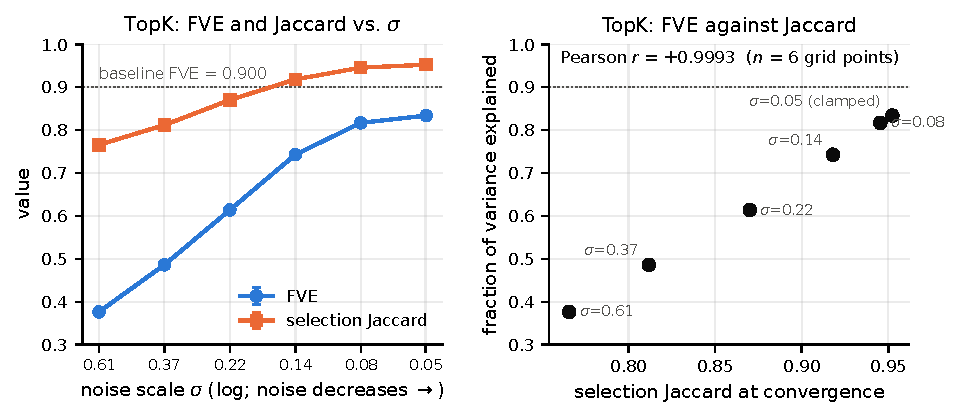
\includegraphics[width=\textwidth]{a2_dose_response.pdf}
\caption{TopK: reconstruction quality (FVE) and selection stability
(Jaccard) as a function of the reparameterisation noise scale, 13 seeds/point
(left; both are fractions, so they share one axis), and FVE against Jaccard
across the six grid points (right), $r=+0.9993$. Error bars are $\pm1$
SD across seeds and are mostly smaller than the markers.}
\label{fig:a2}
\end{figure}

\subsection{Generalises to a globally-shared selection budget}

Is this a property of \emph{per-token} hard selection specifically, or of
hard cardinality constraints more generally? BatchTopK~\citep{bussmann2024batchtopk}
selects the global top-$(k\cdot\mathrm{batch\_size})$ activations over an
entire flattened batch rather than exactly $k$ per token, so one token's
noise-promoted feature can in principle be compensated by another token's
correspondingly demoted one --- the natural candidate for ``more
noise-robust,'' since the selection budget is more elastic.

Repeating the identical six-point sweep on \texttt{VSAEBatchTopK} (matched
$d$, $k$, hook point, and training schedule; two pre-existing
saved-checkpoint bugs found and fixed en route, \S\ref{app:bugs}) gives an
essentially identical coupling: $r(\mathrm{FVE},\mathrm{Jaccard}) = +0.9979$
(Table~\ref{tab:a3}, Figure~\ref{fig:a3}), against TopK's $+0.9993$. If
anything the more flexible selection rule is \emph{slightly more} exposed to
noise at matched sigma, not less: comparing each architecture's own FVE as a
fraction of its own (higher) deterministic baseline, BatchTopK recovers a
consistently smaller fraction than TopK at every one of the six matched noise
scales (e.g., $90.3\%$ vs.\ $92.6\%$ of baseline at the clamp floor), the
opposite of the ``elastic budget'' intuition's prediction.

\begin{table}[h]
\centering
\caption{BatchTopK: the same sweep. Deterministic baseline FVE $=0.9509\pm0.0004$.}
\label{tab:a3}
\begin{tabular}{lcccc}
\toprule
$\log\sigma^2_{\mathrm{init}}$ & $\sigma$ (effective) & FVE & Jaccard \\
\midrule
$-1.0$ & $0.6065$ & $0.3434 \pm 0.0035$ & $0.6969 \pm 0.0042$ \\
$-2.0$ & $0.3679$ & $0.4787 \pm 0.0074$ & $0.7546 \pm 0.0078$ \\
$-3.0$ & $0.2231$ & $0.6179 \pm 0.0046$ & $0.8348 \pm 0.0030$ \\
$-4.0$ & $0.1353$ & $0.7553 \pm 0.0015$ & $0.8912 \pm 0.0004$ \\
$-5.0$ & $0.0821$ & $0.8391 \pm 0.0010$ & $0.9222 \pm 0.0003$ \\
$-8.0$ (clamped) & $0.0498$ & $0.8588 \pm 0.0007$ & $0.9311 \pm 0.0003$ \\
\bottomrule
\end{tabular}
\end{table}

\begin{figure}[t]
\centering
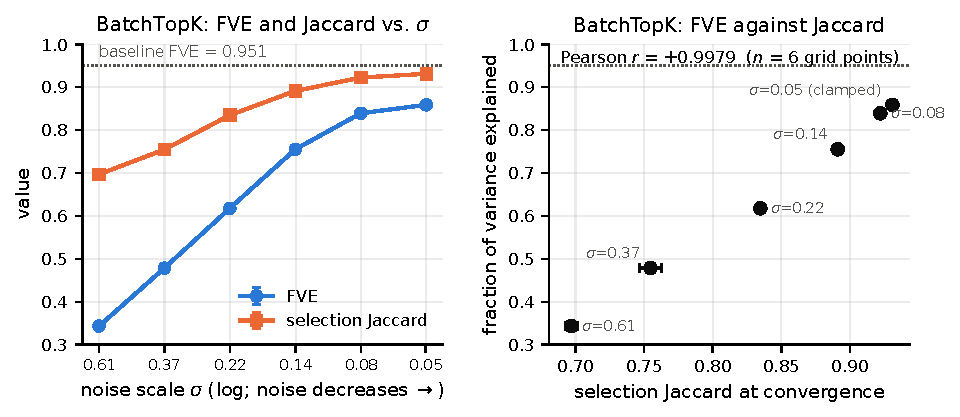
\includegraphics[width=\textwidth]{a3_batchtopk_dose_response.pdf}
\caption{BatchTopK: the same dose-response, $r=+0.9979$.}
\label{fig:a3}
\end{figure}

The mechanism therefore does not depend on strict per-token selection: it
looks like a property of hard, cardinality-constrained selection under noise
in general, established here on two architectures that share that property
despite scoping their selection budgets differently.

\subsection{Breaks down for a soft, gradient-learned threshold}

JumpReLU~\citep{rajamanoharan2024jumprelu} replaces Top-K's hard cardinality
constraint with a per-feature learned threshold and a soft
sparsity-target loss, trained via a straight-through
estimator~\citep{bengio2013estimating}. No sparsity budget is enforced
architecturally; achieved sparsity is whatever the threshold, trained by
gradient descent against an $L_0$-target penalty, converges to. This is the
sharpest available test of whether the mechanism found above depends on
\emph{hard-$k$ selection specifically} or on \emph{discreteness of selection
in general}: JumpReLU is discrete (a feature is either gated on or off) but
not hard-$k$.

No training script for the variational JumpReLU trainer in this codebase had
ever been exercised end to end; building one and running the identical
six-point sweep surfaced three functional bugs that had to be fixed before
any measurement was meaningful (a dead gradient on the threshold parameter,
a missing sparsity-target loss term, and --- the one that would have made
this experiment structurally impossible to run at all --- a gate that was
applied \emph{before} sampling rather than after, meaning noise could only
perturb the value of an already-selected feature and could never change the
selected set; \S\ref{app:bugs} gives the full account). With all three fixed
and verified (repeated forward passes on one token show real selection churn,
mean Jaccard $0.35$, after the fix, versus $1.0$ --- no churn possible ---
before it), the same six-point sweep gives Table~\ref{tab:a4}.

\begin{table}[h]
\centering
\caption{JumpReLU: the same sweep, plus achieved $L_0$ (target: 256, matching
$k$). Deterministic baseline FVE $=0.9210\pm0.0003$, $L_0=269.4$.}
\label{tab:a4}
\begin{tabular}{lccccc}
\toprule
$\log\sigma^2_{\mathrm{init}}$ & $\sigma$ & $L_0$ & FVE & Jaccard \\
\midrule
$-1.0$ & $0.6065$ & $36.8$ & $0.3967 \pm 0.0022$ & $0.9637 \pm 0.0009$ \\
$-2.0$ & $0.3679$ & $98.2$ & $0.5346 \pm 0.0022$ & $0.9635 \pm 0.0004$ \\
$-3.0$ & $0.2231$ & $290.8$ & $0.7461 \pm 0.0016$ & $0.9779 \pm 0.0002$ \\
$-4.0$ & $0.1353$ & $247.2$ & $0.7979 \pm 0.0008$ & $0.9913 \pm 0.0006$ \\
$-5.0$ & $0.0821$ & $261.2$ & $0.8522 \pm 0.0008$ & $0.9883 \pm 0.0003$ \\
$-8.0$ & $0.0498$ & $265.0$ & $0.8632 \pm 0.0006$ & $0.9867 \pm 0.0003$ \\
\bottomrule
\end{tabular}
\end{table}

\begin{figure}[t]
\centering
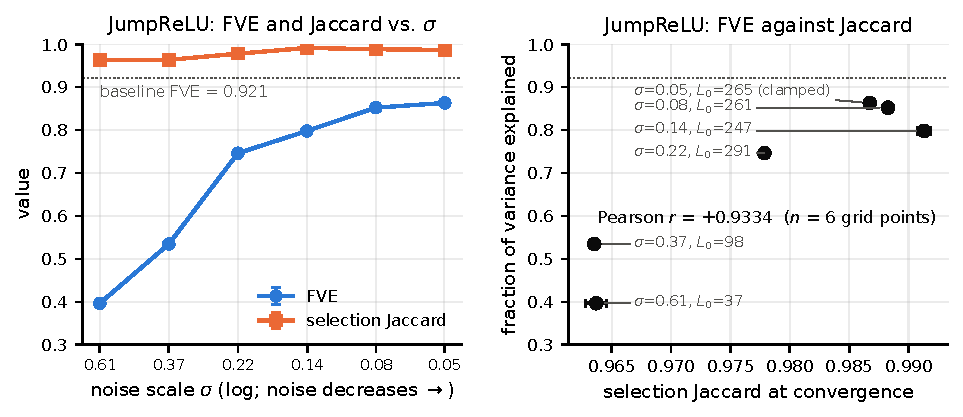
\includegraphics[width=\textwidth]{a4_jumprelu_dose_response.pdf}
\caption{JumpReLU: the same sweep, with each point's achieved $L_0$ shown
beside its noise scale. The naive $r=+0.9334$ annotated on this figure is
confounded by that $L_0$ variation (\S\ref{sec:a4confound}); it is superseded
by the $L_0$-controlled reading in the text.}
\label{fig:a4}
\end{figure}

\subsubsection{The naive coupling number is confounded}
\label{sec:a4confound}

Read naively, $r(\mathrm{FVE},\mathrm{Jaccard})=+0.9334$ over these six points
looks like a slightly looser version of the same TopK/BatchTopK finding.
It is not a clean replication, for a reason Table~\ref{tab:a4}'s third column
makes visible: achieved $L_0$ swings from $36.8$ to $290.8$ --- an
$8\times$ range, non-monotonic in $\sigma$ --- because heavy noise pushes
pre-activations below threshold faster than the soft sparsity loss's
gradient can pull the threshold down to compensate. TopK and BatchTopK hold
sparsity \emph{exactly} fixed at every grid point by construction, so Jaccard
is the only thing varying across their grids and their tight correlations are
a clean read of ``selection churn costs reconstruction at fixed sparsity.''
JumpReLU offers no such guarantee, and $r(\mathrm{FVE}, L_0) = +0.9494$ across
the same six points --- as tight as, or tighter than, $r(\mathrm{FVE},
\mathrm{Jaccard})$ --- so the naive number cannot distinguish ``selection
churn hurts reconstruction'' from ``noise is crushing the achieved
active-feature count, and a 37-feature dictionary reconstructs worse than a
265-feature one for reasons that have nothing to do with \emph{which} 37 or
265 features they are.''

Restricting to the four grid points where achieved $L_0$ sits in a comparable
band to the 256 target ($\log\sigma^2_{\mathrm{init}}\in\{-3,-4,-5,-8\}$,
$L_0\in[247,291]$) --- the closest approximation this soft-target design
allows to TopK/BatchTopK's fixed-sparsity comparison --- the coupling
weakens sharply: $r(\mathrm{FVE},\mathrm{Jaccard})$ drops to $+0.6297$
($n=4$), and $r(\mathrm{FVE}, L_0)$ on the same four points is $-0.5467$
(wrong sign). The relationship is also non-monotonic in a way the hard-$k$
architectures never showed: Jaccard rises from $0.9779$ to a peak of $0.9913$
at $\log\sigma^2_{\mathrm{init}}=-4$ and then \emph{falls} at $-5$ and $-8$
even as $\sigma$ keeps decreasing, while FVE keeps climbing through the same
region --- the two curves visibly decouple exactly where $L_0$ is held
roughly constant.

\subsubsection{Follow-up: densifying the grid rules out a small-$n$ artifact}
\label{sec:a4followup}

Four confound-controlled points is not enough on its own to tell ``the
coupling genuinely weakens'' from ``this design cannot see it.'' The
thing under-powered was grid \emph{coverage} in the $L_0$-matched region,
not per-point precision, so we added four new noise-scale points
($\log\sigma^2_{\mathrm{init}}\in\{-3.5,-4.5,-5.5,-6.0\}$) filling exactly
the gap the original grid's integer spacing left unsampled between $-3$ and
$-8$, at 5 seeds/arm --- a deliberately scoped-down follow-up (lower
per-point seed count than the main battery, honestly reported as such; each
new point's own mean is still precise to 3--4 decimals, e.g.\
$\log\sigma^2_{\mathrm{init}}=-6.0$: FVE $0.8632\pm0.0010$, $L_0$
$265.1\pm0.4$, Jaccard $0.9868\pm0.0004$). On the widened $L_0$-matched
band this requires ($L_0\in[247,315]$, eight points:
$\log\sigma^2_{\mathrm{init}}\in\{-3,-3.5,-4,-4.5,-5,-5.5,-6,-8\}$):
\begin{equation*}
r(\mathrm{FVE},\mathrm{Jaccard}) = +0.5026 \ (n=8) \qquad
r(\mathrm{FVE}, L_0) = -0.4704 \ (n=8),
\end{equation*}
against the original four-point reading's $+0.6297$ and $-0.5467$. Both
correlations move modestly and in a direction consistent with sampling
noise on a still-small $n$, not a systematic reversal, and the full
ten-point grid's naive coupling is essentially unchanged by the denser
sampling ($r=+0.9341$ vs.\ the six-point grid's $+0.9334$; $r(\mathrm{FVE},
L_0)=+0.9245$ vs.\ $+0.9494$). This is the evidence the original four-point
design could not supply on its own: \textbf{doubling the grid density in
exactly the region where achieved sparsity is held roughly fixed reproduces
the same qualitative pattern}, so the weakened coupling is not an artifact
of having too few confound-controlled points to trust.

\begin{figure}[t]
\centering
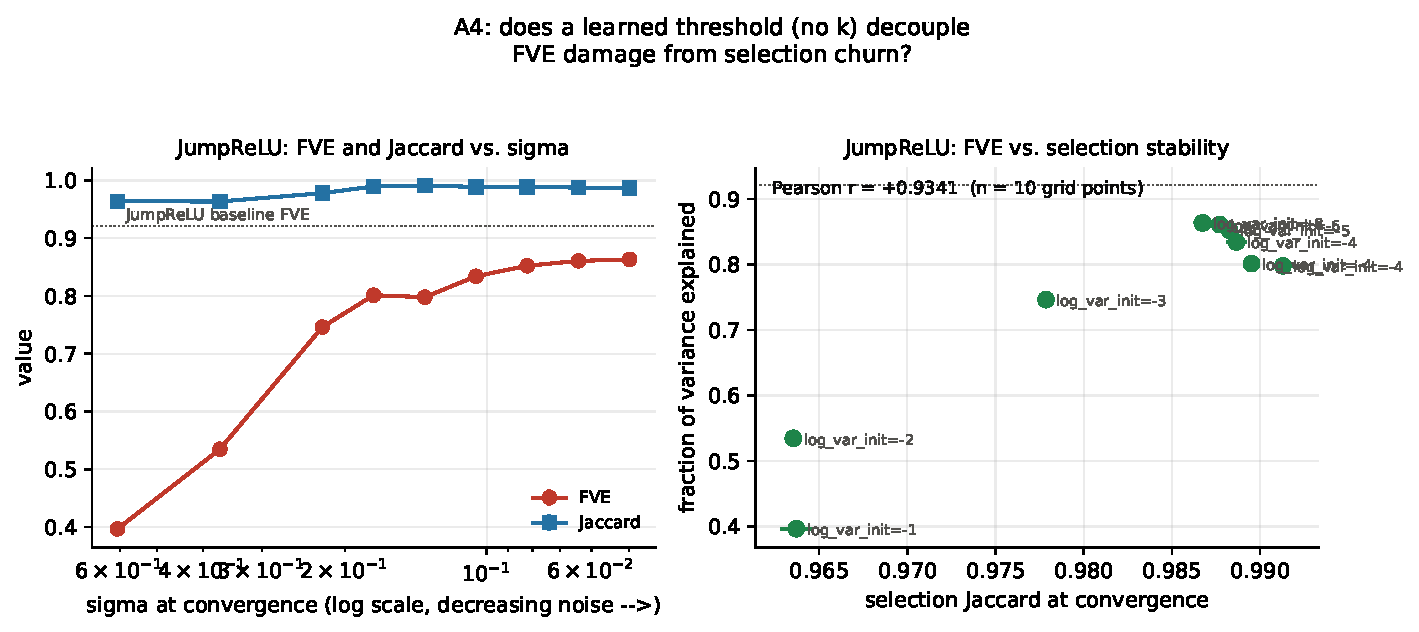
\includegraphics[width=\textwidth]{a4_followup_dose_response.pdf}
\caption{JumpReLU with the four densifying points added (ten total; the four
new points at $\log\sigma^2_{\mathrm{init}}\in\{-3.5,-4.5,-5.5,-6.0\}$ are
5-seed means). The naive $r=+0.9341$ annotated on this figure is confounded
by achieved-sparsity variation in the same way as the original six-point
figure (Figure~\ref{fig:a4}); the $L_0$-matched, confound-controlled reading
is $r=+0.5026$ ($n=8$), reported in the text.}
\label{fig:a4followup}
\end{figure}

\subsubsection{What this licenses}

The question as posed --- ``does the same tight FVE-vs-selection-churn
coupling hold for a soft, no-$k$-at-all selection mechanism?'' --- gets a
clearer answer than the original four-point design alone could give: no,
and this is now backed by twice the grid coverage in the region where the
comparison is meaningful. \S\ref{sec:a4followup}'s $n=8$ reading does not
turn this into a clean null in the formal sense --- both correlations are
still nonzero, and eight points remains a small-$n$ correlation by the
standards of \S\ref{sec:mechanism}'s own permutation-test comparisons
elsewhere in this paper --- but it rules out the specific alternative
explanation that the original four-point reading was a fluke of only four
points. What the experiment licenses is a different, and arguably more
basic, finding than the one it was designed to detect: \emph{a soft,
gradient-learned threshold's achieved sparsity level, not just its
selection stability, is not noise-robust}. TopK and BatchTopK cannot
exhibit this failure mode by construction --- their cardinality constraint
is architectural, not learned --- so a soft-threshold mechanism under
sampling noise fails in a qualitatively different way from a hard-$k$ one,
not merely a quantitatively noisier version of the same failure.

\subsection{Synthesis}

Put together, \S\ref{sec:mechanism} supports a claim sharper than
``reparameterisation is incompatible with discrete Top-K selection'': the
amount of Top-K-style selection churn a given noise scale induces predicts,
almost linearly, how much reconstruction quality it costs, across a $12\times$
range of noise and across two architectures that scope their hard
cardinality constraint differently (per-token vs.\ globally-shared). There is
no threshold effect and no ``free'' amount of noise on either architecture
--- only a continuum, with the residual gap at the achievable floor exactly
the size the floor's own sigma predicts. A soft selection mechanism is not a
smoother version of the same story; it introduces a second failure axis
(achieved sparsity itself, not just which features are selected) that a hard
cardinality constraint cannot have. The constructive reading, echoing why
Gumbel-Softmax~\citep{jang2016categorical} and the Concrete
distribution~\citep{maddison2016concrete} exist as a response to exactly this
tension between continuous relaxations and discrete selection: \emph{if the
goal is a stochastic sparse code, the noise belongs in the selection
decision, not in the magnitude of an already-selected feature.} Every vSAE
construction examined here does the opposite.

\section{Reported effect sizes as a lower bound on implementation variance}
\label{sec:variance}

Section~\ref{sec:e1}'s decomposition identified five implementation details
--- a KL warmup schedule, a bias parameterisation, an initial decoder scale,
a decoder-gradient-projection omission, and an initial weight distribution
--- that, individually, moved a standard liveness metric enough to be
detected at $5\sigma$ with 13 seeds/arm, and none of which appears in either
implementation's stated loss equation. A sixth, independent example
sharpens the same point without touching the KL term at all: the released
vSAE trainer applies \texttt{F.relu(mu)} to its posterior mean before the
reparameterisation step; a second trainer in the same codebase, built to
mask the KL term to only the Top-K-selected features as a direct test of the
preprint's stated feature-death mechanism, does not. Neither published
paper's equations show a ReLU here. Run as its own two-arm factor (13 seeds,
holding everything else fixed):

\begin{table}[h]
\centering
\caption{The unremarked \texttt{F.relu(mu)}: one line, $d\approx15$--$19$, $5.03\sigma$.}
\label{tab:e3}
\begin{tabular}{lcc}
\toprule
Threshold & no-ReLU (as in preprint equations) & ReLU (as in released code) \\
\midrule
$<0.1\times k/d$ & $0.1315 \pm 0.0074$ & $0.0287 \pm 0.0033$ ($d=+19.3$) \\
$<0.5\times k/d$ & $0.4655 \pm 0.0113$ & $0.3081 \pm 0.0092$ ($d=+15.3$) \\
\bottomrule
\end{tabular}
\end{table}

Both thresholds agree in direction, so this is a robust effect, not a shape
change: adding the ReLU cuts the near-dead-feature population by a factor of
$\sim4.6$ at the tight threshold. Had either trainer simply been patched to
match the other, as is routine practice when reconciling two implementations
of ``the same'' model, every subsequent number computed from that trainer
would have silently inherited a $d\approx15$--$19$ effect misattributed to whatever
the actual comparison of interest was.

Table~\ref{tab:variance} collects every implementation-level factor measured
in this paper. None of them is a hyperparameter anyone tunes, reports, or
ablates in a typical SAE paper; all six are default behaviour, one line of
code, and invisible in a state dict or a loss equation.

\begin{table}[h]
\centering
\caption{Six one-line implementation details and their individually-measured
effect sizes, all significant at $5.03$--$5.16\sigma$ (13 seeds/arm). For
reference, published architectural claims in this literature are typically
reported without seed variance at all (\S\ref{sec:seedsurvey}); a $d>10$
implementation effect is larger than most reported architectural ones.}
\label{tab:variance}
\begin{tabular}{lcc}
\toprule
Detail & Metric moved & $|d|$ \\
\midrule
KL warmup schedule + bias parameterisation (combined) & liveness (loose) & $13.0$ \\
Initial decoder scale & FVE & $16.5$ \\
Decoder-gradient-projection omission & FVE & $3.8$--$14.3^{*}$ \\
Initial decoder-weight distribution (Gaussian vs.\ uniform) & FVE, frac.\ recovered & $4.7$, $7.3$ \\
\texttt{F.relu(mu)} presence/absence & liveness & $15.3$--$19.3$ \\
\bottomrule
\end{tabular}

\vspace{2pt}
\footnotesize{$^{*}$Reported as a single factor in two different comparison
contexts (against different upstream generations of the ladder); both values
are real, significant effects, not a range of uncertainty.}
\end{table}

\subsection{The decoder-gradient-projection effect does not generalise to a penalty-free Top-K SAE}
\label{sec:claim4}

Table~\ref{tab:variance}'s largest entry after the ReLU, the
decoder-gradient-projection omission, was discovered and measured entirely
within the vSAE family: every arm in Table~\ref{tab:e1ladder} carries a
nonzero activation penalty (the vSAE's KL term, or its $L_2$-penalty null
model). This leaves open whether the effect is a generic, unremarked factor
in Top-K SAE training that any two independently-implemented Top-K SAEs
could differ on, or an interaction specific to training alongside a
penalty/KL term. We tested this directly: the trainer that produces this
paper's clean Top-K baseline (\S\ref{sec:e1}'s null model with its penalty
set to zero) hardcoded the projection unconditionally; we added a config
flag (default \texttt{True}, so every existing checkpoint's behaviour is
unchanged) and trained a new arm identical to the baseline in every other
respect with the projection turned \emph{off}, 13 seeds.

\begin{table}[h]
\centering
\caption{Turning the same projection off in a plain, penalty-free Top-K SAE:
null on every metric, both liveness thresholds agreeing (13 seeds/arm,
$5.16\sigma$ floor).}
\label{tab:claim4}
\begin{tabular}{lccc}
\toprule
Metric & projection on (baseline) & projection off & $d$ ($p$) \\
\midrule
FVE & $0.900159 \pm 0.0006$ & $0.900009 \pm 0.0005$ & $+0.3$ ($p=0.50$) \\
frac.\ recovered & $0.964336 \pm 0.0005$ & $0.964065 \pm 0.0006$ & $+0.5$ ($p=0.22$) \\
$<0.1\times k/d$ & $0.754169 \pm 0.0013$ & $0.753794 \pm 0.0014$ & $+0.3$ ($p=0.53$) \\
$<0.5\times k/d$ & $0.754357 \pm 0.0014$ & $0.754056 \pm 0.0013$ & $+0.2$ ($p=0.63$) \\
\bottomrule
\end{tabular}
\end{table}

Nothing moves detectably, at the identical statistical power ($13$ seeds,
$5.16\sigma$ floor) that detected $d=+3.8$ to $+16.5$ effects of the
\emph{same} one-line change inside the vSAE family. This answers the
question directly, and narrows rather than weakens the claim
Table~\ref{tab:variance} makes: the decoder-gradient-projection effect is
real, large, and undocumented in either paper's equations, but its scope is
models carrying an activation penalty, not Top-K SAE training in general. A
plain Top-K SAE and an independently-implemented plain Top-K SAE that differ
only on this one line would not, on this evidence, be expected to differ
measurably; a vSAE (or an $L_2$-penalised Top-K SAE) and one that differs
only on this line would. This is itself informative about \emph{why} the
effect exists: it is consistent with an interaction between the projection
and the penalty term's own gradient contribution, not with the projection
mechanically mattering to decoder-norm renormalisation on its own, which
would have shown up here too. (We did not find a below-threshold trend in
either direction to further motivate that mechanism; the result is a clean
null, not a smaller-but-present effect.)

\subsection{A design-level point this implies}
\label{sec:seedsurvey}

None of these effects required an unusual amount of statistical power to
detect; they were detected at the same power ($13$ seeds/arm, $5.03$--
$5.16\sigma$) used throughout this paper. The combinatorial floor on that
power is worth stating plainly, because it caps what \emph{any} design with
fewer seeds can claim, regardless of the underlying effect size. A two-sided
seed-permutation test's minimum attainable $p$-value is $2/\binom{2n}{n}$
for $n$ seeds per group (Table~\ref{tab:seedceiling}): at $n=6$ that floor is
$p=0.00216$, i.e.\ $3.07\sigma$ --- not because the effect is small, but
because the design cannot express more evidence than that, however large
$d$ actually is. Thirteen seeds per group is the first $n$ at which this
floor drops below the conventional $5\sigma$ threshold; at $n=1$, the floor
is $p=1$ ($0\sigma$) --- a single-seed design cannot express \emph{any}
level of statistical significance for a claim of the form ``architecture A
beats architecture B,'' independent of how large the true effect is.

\begin{table}[h]
\centering
\caption{The sigma ceiling of a two-sided seed-permutation test, by seeds
per group. Same formula ($2/\binom{2n}{n}$) as every confirmatory
comparison in this paper.}
\label{tab:seedceiling}
\begin{tabular}{lcccccccc}
\toprule
$n$/group & 1 & 2 & 3 & 5 & 6 & 10 & 13 & 20 \\
\midrule
sigma ceiling & $0.00$ & $0.97$ & $1.64$ & $2.65$ & $3.07$ & $4.40$ & $5.21$ & $6.75$ \\
\bottomrule
\end{tabular}
\end{table}

We checked how large this gap actually is by surveying every SAE-methods
paper cited in this paper's own related work (\S\ref{sec:related}) --- a
sampling frame fixed by that bibliography, not curated for this
subsection --- for how many independently-seeded training runs each
reports for a single hyperparameter configuration
(Table~\ref{tab:seedsurvey}). \textbf{Ten of ten report exactly one.} The
one exception found anywhere in the survey ---
\citet{bricken2023monosemanticity}'s second, independently-seeded
transformer --- is used only for a qualitative feature-universality check,
not the paper's main quantitative claims, and its own $n=2$ sits below the
conventional $p<0.05$ threshold regardless. Several of these papers train
\emph{many} SAEs (SAEBench trains ``over 200''
\citep{karvonen2025saebenchcomprehensivebenchmarksparse}; JumpReLU trains
``multiple 131k-width SAEs... of each type''
\citep{rajamanoharan2024jumprelu}), but as a sweep over hyperparameters ---
width, sparsity, architecture --- not as repeated seeds of one
configuration; that breadth buys coverage across the hyperparameter space,
not statistical power for any single comparison within it.

\begin{table}[h]
\centering
\caption{Independently-seeded training runs per configuration, surveyed
across every SAE-methods paper this paper cites. Full text of each paper
searched via its arXiv HTML (two Anthropic/Transformer-Circuits posts
exceeded a direct-fetch size limit; those two entries rest on multiple
independent web searches quoting the papers' own methodology instead, and
are flagged as such).}
\label{tab:seedsurvey}
\begin{tabular}{lc}
\toprule
Paper & seeds/configuration \\
\midrule
\citet{cunningham2023sparse} & 1 \\
\citet{bricken2023monosemanticity} & 1 (2 for one supplementary check only)$^{*}$ \\
\citet{templeton2024scaling} & 1$^{*}$ \\
\citet{gao2024scalingevaluatingsparseautoencoders} & 1 \\
\citet{rajamanoharan2024gated} & 1 \\
\citet{rajamanoharan2024jumprelu} & 1 \\
\citet{bussmann2024batchtopk} & 1 \\
\citet{karvonen2025saebenchcomprehensivebenchmarksparse} & 1 \\
\citet{marks2025sparsefeaturecircuitsdiscovering} & 1 \\
\citet{lu2025sparseautoencodersagain} & 1 \\
\bottomrule
\end{tabular}

\vspace{2pt}
\footnotesize{$^{*}$Not backed by a direct full-text fetch; see caption.}
\end{table}

One nuance is worth stating precisely rather than flattening: JumpReLU
\emph{does} report binomial confidence intervals for a manual human-
interpretability rating study \citep{rajamanoharan2024jumprelu} ---
evaluation-level uncertainty, not training-seed-level uncertainty. This is
exactly the distinction \S\ref{app:stats} draws (a token- or rater-level
test estimates evaluation noise and cannot support an architecture-level
claim) showing up unprompted in the surveyed literature: eval-level
uncertainty quantification is not rare here; architecture-level (seed)
uncertainty, this survey suggests, is close to absent.

This gap is not merely theoretical. Two papers outside the survey above ---
they measure seed \emph{sensitivity} itself, not the field's reporting
practice, so they are not part of Table~\ref{tab:seedsurvey} --- found
substantial seed-to-seed instability in exactly the object a single-seed
design cannot detect. \citet{paulo2025sae} found only $\sim30\%$ feature
overlap between two otherwise-identical $131$k-latent SAEs differing only
in random seed (Llama-3-8B, replicated across multiple layers, LLMs, and
datasets); \citet{gerasimov2026unstable} found individual features vary
substantially across seeds in a large-scale multi-seed study, though they
cluster into reproducible lower-rank subspaces. Neither result was designed
to be detectable by any of the ten papers surveyed above, and both found
it anyway once someone looked.

Every effect size in this paper is real in the sense that it survived a
design capable of expressing $5\sigma$; the implementation choices
catalogued in Table~\ref{tab:variance} are large enough that a design
matching the field's own modal practice ($n=1$) could not, even in
principle, distinguish them from the architectural effect a comparison was
nominally about --- not because those studies' point estimates are wrong,
but because a claim of the form ``architecture A beats architecture B''
is not a claim a single-seed design can license, independent of the true
effect size.

\section{A case study in metric disagreement: SCR and TPP on the same checkpoints}
\label{sec:e4}

The preceding sections establish what the KL term and the reparameterisation
trick do to reconstruction and to the dictionary's own internal liveness
statistics. A separate, harder question is whether any of this changes what
downstream interpretability benchmarks report. We do not resolve this
question in this paper; we report it as a worked example of a problem that
generalises beyond this specific comparison.

\subsection{The comparison and the first disagreement}

Two recovered Pythia-70M checkpoints from the original preprint this
codebase extends --- a Top-K baseline ($d=8192$, AuxK $\alpha=0.03125$) and
its corresponding vSAE ($\beta=1$, fixed variance, AuxK \emph{off},
$1{,}474/8192$ live features) --- were scored with SAEBench's spurious
correlation removal (SCR) and targeted probe perturbation (TPP) metrics
\citep{karvonen2025saebenchcomprehensivebenchmarksparse} on the same
dataset (\texttt{bias\_in\_bios}, professor/nurse) and the same
size-response design: mask the baseline dictionary down to a grid of $N$
features by usage frequency, score each point, and compare the vSAE's own
(unmasked, natural) score against the resulting curve at $N=1{,}474$. SCR
is SAEBench's adaptation of the earlier SHIFT
protocol~\citep{marks2025sparsefeaturecircuitsdiscovering} (ablate
SAE latents a probe identifies as encoding a spurious attribute, and
measure how much target-concept accuracy survives); TPP extends the same
idea to simultaneous multi-class disentanglement.

\begin{table}[h]
\centering
\caption{SCR and TPP disagree on the same two checkpoints, same dataset,
same grid.}
\label{tab:e4}
\small
\begin{tabular}{lccc}
\toprule
Metric & vSAE score & baseline curve at $N=1474$ (\texttt{top\_usage}) & margin \\
\midrule
SCR & $0.1017$ & $0.0201$ & $+0.082$ (not explained by size) \\
TPP & $0.1055$ & $0.1905$ & $-0.085$ (explained by size) \\
\bottomrule
\end{tabular}
\end{table}

SCR says the vSAE's advantage over its baseline is not explained by
dictionary size (its unmasked score clears every point on the masked curve,
including the top-usage reference and a bracket of 90 random-subset draws).
TPP says the opposite: the vSAE's score sits \emph{below} both the top-usage
and the random-subset references at the same $N$. This is not a subtle
effect that disappears under scrutiny; it is a sign flip on the exact same
comparison, and it recurs in every diagnostic we ran against it.

\subsection{Five diagnostics, none of which explains the disagreement away}
\label{sec:e4discussion}

We treated the disagreement as a claim requiring its own falsification
attempt and ran five diagnostics, roughly cheapest-to-test first.

\begin{enumerate}
\item \textbf{Is the mean-across-thresholds summary hiding a shape change?}
  Both scorers' internal per-threshold breakdown ($N\in\{2,5,10,20\}$
  ablated features) was extended and re-derived. SCR says ``not explained''
  at all four thresholds; TPP says ``explained'' at all four, though
  decisively only at $N\le10$ (a near-tie at $N=20$). The disagreement is not
  an artifact of averaging.
\item \textbf{Is it a test-set-noise artifact?} A 200-draw bootstrap of the
  cached test set (conditional on node effects fixed from the full train
  set) leaves both mean margins clearing zero in opposite directions: SCR
  $+0.082$ $[+0.024,+0.150]$, TPP $-0.086$ $[-0.090,-0.081]$. SCR's interval
  is $\sim15\times$ wider than TPP's and, per-threshold, clears zero only at
  $N=2$; a full bootstrap that also re-derives node effects from a
  train-set resample widens SCR's interval further ($+0.088$
  $[+0.008,+0.171]$) but still does not cross zero. The disagreement
  survives resampling, though the two sides are not equally sturdy.
\item \textbf{Do the two metrics select systematically different features?}
  A falsifiable prediction --- SCR's top-effect features should rank low in
  usage frequency, TPP's should rank high, since disentangling a correlated
  pair plausibly needs a rare feature while separating many classes needs
  broad ones --- was stated in advance and tested by reading which features
  each metric's own effect computation ranks highest, cross-referenced
  against their usage-percentile rank. It is falsified: both metrics' top
  features sit in the same $0.55$--$0.73$ usage-percentile band at every
  $N$, the small gap between them flips sign between $N\le5$ and $N\ge10$,
  and within-metric variance across classes dwarfs any between-metric
  difference.
\item \textbf{Does it generalise across datasets and class pairs?} Extending
  to three more \texttt{bias\_in\_bios} pairs and a second SAEBench dataset
  (Amazon reviews) finds both verdicts replicating as the dominant pattern,
  not reversing: SCR ``not explained'' on 7 of 8 (dataset, pair) points; TPP
  ``explained'' via its top-usage reference on both datasets, though its
  random-subset reference goes from decisive to a coin flip on the second
  dataset.
\item \textbf{Is the masked reference curve itself the wrong comparison?}
  Every point on the masked curve is the \emph{same} baseline dictionary
  with entries zeroed post hoc; the vSAE's 1,474 live features were learned
  together, and a dictionary trained from scratch at that exact size might
  organise its capacity differently. Training a real Top-K SAE at
  $\mathrm{dict\_size}=1474$ (otherwise identical config) and scoring it
  directly against the original professor/nurse point finds its SCR score
  ($0.020127$) matches the masked curve's reference ($0.020127$) to
  $6\times10^{-8}$, and its TPP score ($0.2025$) is slightly \emph{higher}
  than the masked reference ($0.1905$) --- on that one point, this specific
  confound is not live. It is not this well-behaved everywhere: scoring the
  same trained-from-scratch checkpoint against the other 7 (dataset, pair)
  points item 4 added finds the reference-curve shift is often substantial
  for SCR (mean absolute shift $0.075$, up to $0.138$ at one point,
  comparable to the margins the verdict rests on) and flips one of eight
  points' individual sign (Software/Electronics, $+0.110\to-0.027$).
  \textbf{The aggregate verdict is essentially unmoved regardless}: the mean
  margin under the trained-small reference ($+0.079$) is marginally
  \emph{larger} than under the masked reference ($+0.072$) on the same
  eight points, and 6 of 8 (was 7 of 8) still say ``not explained.'' TPP's
  two available points (bias\_in\_bios, amazon; TPP has no per-pair concept)
  both keep their ``explained by size'' verdict under the trained-small
  reference. The honest summary is narrower than the single-point reading:
  the masking-vs-training confound is real and can move an individual
  pair's verdict, but it does not systematically favour either metric's
  side, so it does not explain the SCR/TPP disagreement itself. (A
  secondary finding en route, from the original point: even given the
  vSAE's exact live-feature count as its budget, a plain Top-K network
  trained at that size keeps only $65.5\%$ of it alive --- matching a
  feature \emph{count} does not guarantee matching how efficiently a
  network uses it.)
\end{enumerate}

\subsection{What we take this to show}

We do not have an explanation for why SCR and TPP disagree here, and we are
explicit that this section does not supply one. What we can report is that
every mechanism we could think of to explain the disagreement away ---
an averaging artifact, sampling noise in the test set, a systematic
difference in which features the two metrics reward, insufficient
generalisation across data, and a masking-vs-training confound in the
reference curve --- fails to do so. One structural difference between the
two metrics' construction is at least consistent with SCR being the noisier
of the two: SCR's per-threshold score is a ratio (divided by
$\mathrm{clean\_acc}-\mathrm{original\_acc}$, which can be small), while
TPP's is a plain difference, and SCR's baseline curve is visibly flatter and
noisier than TPP's own equivalent curve across the same $N$ range. This is
consistent with, but does not establish, part of the disagreement being a
metric-construction property rather than a property of the two dictionaries'
features --- and it does not explain the sign flip itself, since SCR's
mean-level margin still excludes zero under both bootstraps.

We report this as a demonstration of a general problem rather than a
finding specific to this vSAE. The same two checkpoints, the same dataset,
the same day of measurement, and two metrics that are both standard,
published, and widely used, disagree in direction on the same substantive
question. Reporting only one of them --- as is standard practice when a
paper picks the metric that supports its narrative --- would be a true
statement about that one metric and a misleading one about the underlying
claim. We regard the correct response to a finding like this as reporting
the disagreement itself, with its own confound-checking, rather than
resolving it by fiat or by omission.

\paragraph{Independent, more direct evidence has since appeared.}
\citet{chanin2026reliable} audits SCR and TPP against three tests neither
this paper nor SAEBench's own release applied --- reseed noise on fixed
canonical SAEs, correlation with a synthetic benchmark's known ground-truth
quality, and discriminability across a training trajectory --- and finds
both fail basic sanity checks at their canonical settings: SCR and TPP
\emph{decline} over the course of training on the panels tested (implying
an untrained SAE is ``better'' than a trained one), TPP's canonical setting
shows essentially zero correlation with ground-truth quality on synthetic
SAEs, and SCR turns \emph{negatively} correlated with ground-truth quality
at large $N$, ranking a perfect oracle below 11 of 35 trained SAEs tested.
The recommendation is to avoid both at their canonical settings entirely.
This is a different, and more direct, kind of evidence than anything in
this section --- it audits each metric against a ground truth we do not
have access to, rather than checking whether the two metrics agree with
each other --- but it points the same way: neither metric's number should
be read as a settled fact about feature quality. It does not resolve which
verdict this paper's own SCR/TPP disagreement should be believed, if
either; if anything, it weakens confidence in both, which is consistent
with, not contrary to, the position this section already takes.

\section{Discussion}
\label{sec:discussion}

\paragraph{What the three parts add up to.} At fixed variance, adding a KL
term to a Top-K SAE is adding an $L_2$ penalty and nothing else
(\S\ref{sec:e1}); the empirical work needed to state that plainly is
checking that two independent implementations of the identical objective
actually agree, which they do only once five unrelated implementation
choices are matched. Once sampling is switched on, the damage is large and
mechanistically specific: it tracks how much the noise perturbs a hard
selection mechanism's chosen set, not some generic notion of representation
quality, and that mechanism generalises across two architectures that scope
their hard-$k$ constraint differently but breaks down --- in an informative
way, not merely a noisier way --- for a soft, gradient-learned threshold
(\S\ref{sec:mechanism}). Both of these facts about the architecture are, in
this codebase, larger than five one-line implementation details that appear
in no equation the released code's own paper states (\S\ref{sec:variance}).
The composite claim is not ``variational sparse autoencoders do not work''
--- it is that the standard construction (isotropic Gaussian prior, fixed
unit variance, hard Top-K selection) cannot test the hypothesis it is
usually offered in support of, because the noise it introduces interacts
with hard selection in a way that is guaranteed to hurt and never
guaranteed to help.

\paragraph{Constructive payload.} If the goal is genuinely a stochastic
sparse code, \S\ref{sec:mechanism}'s synthesis gives a specific, testable
design recommendation rather than a negative result: put the noise in the
\emph{selection decision} (as Gumbel-Softmax and Concrete relaxations do for
discrete choices generally~\citep{jang2016categorical,maddison2016concrete},
and as \citet{berthet2020learning}'s differentiable perturbed optimisers do
specifically for top-$k$-type discrete selection --- exactly the operation
whose interaction with reparameterisation noise this paper measures ---
by perturbing the ranking \emph{before} the argmax/top-$k$ step and
differentiating through the resulting expectation, rather than perturbing
an already-selected value afterward), not in the magnitude of an
already-selected feature. The hard-concrete stochastic gate of
\citet{louizos2018learning}, developed for $L_0$-regularised weight
sparsity rather than sparse coding, is a close structural cousin: a
continuously-relaxed \emph{gate} decides membership, and a separate
mechanism sets magnitude, which is exactly the separation this paper's
noise-in-selection recommendation asks for and JumpReLU's own architecture
(gate, then value) gestures toward without actually placing the
\emph{noise} at the gate. A prior with mass at zero --- spike-and-slab
being the textbook example for sparse codes, in contrast to the isotropic
Gaussian's zero mass at the origin, and already used for exactly this
purpose in a VAE by \citet{tonolini2020variational} --- is a second,
related direction: it would make the KL term itself do something other
than shrink activation magnitude uniformly. Neither is tested here; both
follow directly from identifying the specific mechanism this paper
measures rather than only its symptom.

\paragraph{A note on the liveness--reconstruction relationship.} An
exploratory (not pre-registered) reading of every replicated arm in this
battery found that reconstruction quality and feature liveness are not a
single trade-off curve: pooled across 11 arms the two metrics look unrelated
($\rho=-0.14$, $p=0.69$), but that null is two opposite-signed relationships
cancelling --- among the subset of arms that reach reasonable reconstruction
quality, better reconstruction buys \emph{more} near-dead features
($\rho=+0.86$, $p=0.007$), the same direction the healthy end of the vSAE
sweeps in this paper's own dose-response curves shows. We flag this only as
context for interpreting Table~\ref{tab:a2}--\ref{tab:a4}'s FVE columns
alongside their own liveness statistics, not as an additional pre-registered
claim.

\subsection{Limitations}

\begin{itemize}
\item \textbf{Single model family for the controlled experiments.} All of
  \S\ref{sec:e1}--\S\ref{sec:variance} runs on GELU-1L-scale residual stream
  activations at one layer, one dictionary size ($4\times d_{\mathrm{model}}$),
  one sparsity level ($k=256$). Whether the decomposition's null result and
  the dose-response's coupling strength hold at larger model or dictionary
  scale is untested here.
\item \textbf{The E4 headline comparison (\S\ref{sec:e4}) carries an
  uncontrolled confound of its own.} The recovered Pythia baseline trains
  with AuxK dead-feature revival on ($\alpha=1/32$); the recovered vSAE
  trains with it off. AuxK is the standard dead-feature mitigation in this
  literature, so the headline ``vastly fewer live features'' comparison
  between these two specific checkpoints confounds the KL term with the
  absence of the standard remedy. This does not affect
  \S\ref{sec:mechanism}'s dose-response sweeps, which hold AuxK fixed
  throughout, but it does affect how strongly \S\ref{sec:e4}'s specific
  numbers should be read as characterising ``the vSAE'' versus
  characterising these two particular checkpoints.
\item \textbf{The noise-scale sweeps (\S\ref{sec:mechanism}) are single-seed
  correlations at the arm level, not a permutation test.} $r=0.9993$,
  $0.9979$, $0.9334/0.6297$ are Pearson correlations over six (or four)
  arm-level means, each itself averaged over 13 seeds; they are strong,
  visually unambiguous relationships, but the unit of statistical inference
  used elsewhere in this paper (a permutation test over seeds) does not
  apply to a six-point curve, and we do not claim $\sigma$-level
  significance for these correlations.
\item \textbf{The JumpReLU result (\S\ref{sec:mechanism}) rests on eight grid
  points after confound control, four of them at reduced seed count.} The
  follow-up in \S\ref{sec:a4followup} rules out $n=4$ being simply too few
  points to trust, but the four new points ran at 5 seeds/arm rather than
  the main battery's 13, and $n=8$ arm-level points is still a small-$n$
  correlation, not a claim carrying the seed-permutation-test guarantees
  \S\ref{app:stats} describes for the rest of this paper. An architectural
  (rather than soft-loss) $L_0$ cap would answer the original question more
  cleanly still, at the cost of turning JumpReLU into another top-$k$
  variant and defeating the point of testing it; not attempted here.
\item \textbf{E4's five diagnostics are single-seed, descriptive readings,
  not a confirmatory battery.} Unlike \S\ref{sec:e1}--\S\ref{sec:variance},
  none of \S\ref{sec:e4}'s numbers come from a pre-registered
  multi-seed design; they establish that a disagreement exists and survives
  several specific attempts to explain it away, not that it would replicate
  at the same statistical standard as the rest of this paper.
\end{itemize}

\section{Related work}
\label{sec:related}

Sparse autoencoders for language-model interpretability were introduced by
\citet{sharkey2022taking} and \citet{cunningham2023sparse}, building on the
superposition hypothesis of \citet{elhage2022superposition} and scaled by
\citet{bricken2023monosemanticity} and, to production-model scale,
\citet{templeton2024scaling}. Top-K sparsity, which this paper's baseline
uses throughout, is due to
\citet{gao2024scalingevaluatingsparseautoencoders}, who also introduce the
AuxK dead-feature revival mechanism this paper's \S\ref{sec:e4} discusses as
a confound. Gated SAEs~\citep{rajamanoharan2024gated}, BatchTopK
\citep{bussmann2024batchtopk} and JumpReLU~\citep{rajamanoharan2024jumprelu}
are, respectively, the sparsity-penalty-side and (for the latter two) the
selection-mechanism-side alternatives this paper's \S\ref{sec:mechanism} and
\S\ref{sec:seedsurvey} draw on; \citet{lu2025sparseautoencodersagain} is a
recent critical re-examination of SAE evaluation practice in the same spirit
this paper's \S\ref{sec:e4} and \S\ref{sec:seedsurvey} are written in.
SAEBench~\citep{karvonen2025saebenchcomprehensivebenchmarksparse} is the
source of the SCR and TPP metrics scored in \S\ref{sec:e4}, and of the
sparse feature circuit evaluation methodology this codebase's downstream
tooling is built on~\citep{marks2025sparsefeaturecircuitsdiscovering}.
\S\ref{sec:seedsurvey}'s survey of these ten papers' own seed-count
practice is corroborated by two independent studies of SAE seed
sensitivity itself, neither part of the survey: \citet{paulo2025sae} found
only $\sim30\%$ feature overlap between otherwise-identical SAEs differing
only in random seed, and \citet{gerasimov2026unstable} found individual
features vary substantially across seeds while clustering into
reproducible lower-rank subspaces. The
variational autoencoder and its reparameterisation
trick~\citep{kingma2013autoencoding} and the $\beta$-weighted KL trade-off
this paper's Eq.~\ref{eq:vsae} follows~\citep{higgins2017betavae} are the two
pieces of machinery this paper's central object combines with Top-K
selection. The straight-through gradient estimator used to make JumpReLU's
threshold trainable~\citep{bengio2013estimating}, the two continuous
relaxations of discrete sampling this paper's constructive discussion points
toward as the right place to put stochasticity in a
selection-based architecture~\citep{jang2016categorical,maddison2016concrete},
and, closer still to top-$k$ selection specifically, the differentiable
perturbed optimisers of \citet{berthet2020learning} and the hard-concrete
stochastic sparsity gate of \citet{louizos2018learning} --- both of which
place noise at the discrete decision itself rather than at an
already-selected value's magnitude, and the latter of which structurally
separates a gate from a magnitude the way JumpReLU's own architecture does,
without placing noise at the gate --- are the closest prior treatments of
the specific tension \S\ref{sec:mechanism} measures: that a continuous
relaxation of a discrete choice and a discrete choice made from
continuously-perturbed inputs are not the same operation, and only one of
them is what a sampled sparse code actually needs.
\citet{tonolini2020variational}'s spike-and-slab VAE is the closest prior
instance of this paper's second constructive suggestion (a prior with mass
at zero), applied to a different sparse-coding setting than Top-K
selection. We are not aware of a prior controlled decomposition of a
variational sparse autoencoder into its constituent implementation choices,
or of a dose-response measurement of the reparameterisation-selection
interaction across multiple selection mechanisms. \citet{chanin2026reliable}
independently audits SCR and TPP against ground-truth and training-
trajectory sanity checks and recommends against both at their canonical
settings; \S\ref{sec:e4} is, to our knowledge, the first report of the two
metrics giving opposite-signed verdicts on the same checkpoints, which is a
different, complementary kind of finding to Chanin's --- disagreement
between two metrics versus failure of either against a ground truth.

\section{Conclusion}
\label{sec:conclusion}

Adding a KL term to a Top-K sparse autoencoder, at the fixed variance every
public implementation we examined actually trains with, adds an $L_2$
activation penalty and nothing else --- verified not merely as algebra but
as an empirical equivalence between two independently-optimised
implementations, once the five unrelated details that initially separated
them are identified and matched. Once sampling is switched on, the resulting
damage has a specific, measurable mechanism --- selection instability under a
hard cardinality constraint --- that generalises across two architectures
scoping that constraint differently and fails informatively, rather than
simply more noisily, for a soft alternative. Both findings required an
amount of implementation-level control that a typical single-seed,
single-implementation SAE comparison does not have, and the implementation
details that turned out to matter are, individually, larger effects than
many of the architectural claims this literature reports without seed
variance at all. We close with a case where our own confound-checking did
not resolve a disagreement between two standard metrics, offered in the
spirit the rest of this paper is written in: a claim is only as good as the
specific alternative explanations that were checked and ruled out, and
absent that checking, a result this literature currently accepts as
supporting evidence for ``variational structure helps'' is, as far as we can
tell, evidence for none of the things it is usually cited for.

\bibliographystyle{plainnat}
\bibliography{references}

\appendix

\section{Statistical methodology}
\label{app:stats}

Every seeded comparison in \S\ref{sec:e1}--\S\ref{sec:variance} is a
two-sided permutation test over training seeds (not tokens, not
checkpoints): the null hypothesis is that arm labels are exchangeable across
the $2n$ seeds in a comparison, and the test statistic is the observed
difference in means. Two combinatorial ceilings bound what such a test can
report, independent of effect size, and every result in this paper states
which one applies.

\paragraph{The seed-count floor.} For $n$ seeds per group, the minimum
attainable two-sided $p$-value under exact enumeration is
$2/\binom{2n}{n}$. At $n=6$ this floor is $p=0.00216$ ($3.07\sigma$); no
effect, however large, can be reported below this floor at $n=6$. At $n=13$
the floor drops to $p=2.5\times10^{-7}$ ($5.16\sigma$) once Monte Carlo
sampling (below) is accounted for, which is why every confirmatory result in
this paper is reported at $5.03$--$5.16\sigma$ rather than an arbitrarily
large significance level: this is the design's own ceiling, not a property
of any particular effect.

\paragraph{The Monte Carlo floor.} Above $\binom{2n}{n}=200{,}000$ possible
assignments ($n>9$ or so, depending on group balance), exact enumeration is
replaced by Monte Carlo sampling of the permutation distribution, whose own
floor is $1/(n_{\mathrm{perm}}+1)$ under the conservative estimator
$(\mathrm{count}+1)/(n_{\mathrm{perm}}+1)$ (the naive $\mathrm{count}/n_{\mathrm{perm}}$
estimator is anti-conservative and can report $p=0$). At the common default
of $n_{\mathrm{perm}}=100{,}000$ this caps evidence at $4.42\sigma$
\emph{regardless of effect size}; every result in this paper instead uses
$n_{\mathrm{perm}}=4{,}000{,}000$ (a vectorised implementation makes this
take under one second), giving a floor of $5.16\sigma$.

\paragraph{The two-threshold liveness rule.} Feature liveness is reported at
two pre-registered thresholds, $<0.1\times k/d$ and $<0.5\times k/d$ of the
architecture's own expected per-feature firing rate, with the rule fixed in
advance: a result counts as robust only if both thresholds agree in
direction; disagreement between them is treated as a positive finding (a
shape change in the usage distribution, not a location shift) rather than
resolved by picking whichever threshold supports the narrative. This rule
caught a genuine shape change --- not a location shift --- twice in the
course of this project's larger confirmatory battery (\S\ref{sec:e1}'s init
factor, and one comparison not otherwise reported in this paper), in both
cases exactly the failure mode a single threshold would have silently
reported as a clean one-directional effect.

\section{The full E1 code diff}
\label{app:e1diff}

Every difference between \texttt{top\_k.py} and \texttt{vsae\_topk.py} (plus
the two training scripts and a third trainer, \texttt{top\_k\_with\_feature\_
penalty.py}, that differs from \texttt{top\_k.py} only by the penalty term),
enumerated by direct code reading and frozen before \S\ref{sec:e1}'s closing
arm ran.

\begin{table}[h]
\centering
\caption{The frozen 15-item code diff behind \S\ref{sec:e1}.}
\label{tab:e1diff}
\begin{tabular}{lp{9cm}}
\toprule
Status & Item(s) \\
\midrule
Matched by config (2) & \texttt{kl\_warmup\_steps}; bias parameterisation \\
Run as a measured factor (2) & decoder init scale; gradient-projection omission \\
No-op, measured (2) & dead-feature-liveness accounting convention; the $\pm10$ pre-selection clamp (never binds: max observed activation $0.194$ against a clamp at $10$) \\
No-op, static (7) & \texttt{abs()} in selection; an unused \texttt{threshold} buffer; the geometric-median initialisation guard; two epsilon/clamp guards; the dead-feature counter update site; a $2.7\%$ initial-norm offset \\
Not a factor by design (1) & RNG consumption order --- the seed itself is the unit of randomisation the permutation design already treats as noise \\
Run as the closing factor (1) & initial decoder-weight distribution (normalised Gaussian vs.\ normalised uniform) --- predicted null, found not null ($d=-4.7$ on FVE) \\
\bottomrule
\end{tabular}
\end{table}

\section{Bugs found and fixed in the course of this work}
\label{app:bugs}

Three checkpoint-affecting bugs and one training-blocking bug set were found
and fixed while producing the results in this paper; we report them because
each one silently altered a reported number before it was found, and because
the corrections change how earlier readings of this same data should be
interpreted.

\paragraph{A checkpoint-save bug corrupted every saved learned-variance
bias.} The routine that rescales a trained model's biases from
normalised-activation space back to raw-activation space at save time
(correct for the encoder and decoder biases) was, until fixed, \emph{also}
applied to the log-variance encoder's bias --- mathematically wrong, since a
log-variance is not on the additive scale that rescaling assumes, and it
drove every saved learned-variance checkpoint's sigma to read as fully
clamp-collapsed regardless of what was actually learned. Corrected (the
log-variance encoder's \emph{weight} is rescaled instead, which is
scale-homogeneous for this quantity), the learned sigma at convergence is a
moderate $\sigma\approx0.27$, not the clamp floor $\sigma=0.0498$ --- the
posterior does not collapse, contrary to an earlier, uncorrected reading of
the same checkpoints. This correction does not change \S\ref{sec:mechanism}'s
dose-response results, which fix $\sigma$ by its \emph{initial} value rather
than reading a learned one, but it does change the interpretation of
\S\ref{sec:e1}--\S\ref{sec:mechanism}'s $\beta=0$ control's own learned
sigma, and an identical bug was independently found and fixed in the
BatchTopK trainer while preparing \S\ref{sec:mechanism}'s BatchTopK sweep.

\paragraph{The official re-evaluation pipeline was checked against an
uncommitted proxy, and the proxy did not replicate.} An early estimate of
how much the bias-correction bug (above) affected officially-reported
reconstruction quality, computed with a standalone proxy script, suggested a
large ($\approx0.12$ FVE) correction. Re-running the actual evaluation
pipeline on every affected checkpoint with the bug corrected found the real
effect is an order of magnitude smaller ($\approx0.005$ FVE); the proxy's
number does not survive contact with the pipeline it was estimating,
although the qualitative claim it was built to support (the posterior does
not collapse) does. Every number reported in \S\ref{sec:e1}--\S\ref{sec:mechanism}
of this paper is from the official pipeline, not the proxy.

\paragraph{Three bugs in the JumpReLU trainer, one of them structural.} As
described in \S\ref{sec:mechanism}: a dead gradient on the threshold
parameter (a non-differentiable comparison where the codebase's own
non-variational JumpReLU trainer already used a straight-through estimator
for exactly this reason); a missing $L_0$-target sparsity loss term (added,
mirroring the non-variational trainer's own); and a gate applied before
sampling rather than after, which would have made this section's central
measurement (selection churn under noise) structurally impossible to observe
at all, since a gate computed before noise is added can never change which
features are selected, only perturb the magnitude of ones already chosen.
The third is a genuine design fork rather than an unambiguous bug --- gating
before sampling is a valid architecture, just a different one, one that
cannot test what \S\ref{sec:mechanism} tests --- and was resolved by
restructuring to match the encode-then-select order the other two
architectures in \S\ref{sec:mechanism} use, so that all three architectures
in that section answer the same question. A fourth, independent bug (decoder
renormalisation not rescaling the learned threshold alongside it, silently
corrupting evaluated output on any non-unit-norm decoder) was also found and
fixed.

\section{Reproducibility}
\label{app:repro}

{\raggedright
All arms in this paper are defined declaratively in this codebase's
\texttt{falsification/run\_arm.py} and trained with
\texttt{python falsification/run\_arm.py -{}-arm <name> -{}-seed <seed>};
\texttt{falsification/preflight.py} validates every arm's wiring without
requiring a GPU. By section:
\begin{itemize}\raggedright
\item \S\ref{sec:e1}: \texttt{e1\_penalty}, \texttt{e1\_vsae\_ref},
  \texttt{e1\_vsae\_ref\_unitinit}, \texttt{e1\_vsae\_ref\_gradproj},
  \texttt{e1\_vsae\_ref\_fullmatch}.
\item \S\ref{sec:mechanism}: \texttt{a2\_sigma\_init\_\{m1,m3,m4,m5\}} plus
  \texttt{e2\_sampling\_only} and \texttt{e2\_sigma\_low\_init} (TopK);
  \texttt{a3\_batchtopk\_*} (BatchTopK); \texttt{a4\_jumprelu\_*} (JumpReLU).
\item \S\ref{sec:variance}: the ReLU factor is \texttt{e3\_masked\_kl} /
  \texttt{e3\_masked\_kl\_relu}; the projection-generalisation control
  (\S\ref{sec:claim4}) is \texttt{baseline} vs.\
  \texttt{claim4\_baseline\_noproj}.
\end{itemize}
Every arm ran at 13 seeds, except \S\ref{sec:a4followup}'s four densifying
JumpReLU points (\texttt{a4\_jumprelu\_sigma\_init\_\{m3\_5,m4\_5,m5\_5,m6\}}),
which ran at 5 (\texttt{falsification/read\_a4\_followup.py}). The
falsification test suite (\texttt{python -m pytest falsification/tests/ -q})
exercises the permutation-test implementation itself, including the
$p$-value floor formulas in \S\ref{app:stats}, and stayed green throughout
this project.\par}

\end{document}
